\chapter{Data Understanding and Preparation}
\label{ch:capitolo1}

The dataset \textit{train.csv} contains 16431 titles of different forms of visual entertainment that have been rated on IMDb, 
an online database of information related to films, television series etc. 
Each record is described by 23 attributes, both numerical and non-numerical. 
% All the variables of the dataset are introduced and explained in Table 1.1 and Table 1.2.


% \section{Distribution of the variables and statistics}\label{sec:variable_distrib}
% This section will give an overview about the distribution of variables that has been carried on to understand patterns, 
% detect meaningful statistics and assess their relevance to the project. 

\section{Discrete attributes}
Table~\ref{tab:attributes} shows the discrete attributes of the dataset,
their types and a brief description of each attribute.
\begin{table}[h]
    \centering
    \begin{tabular}{|l|l|l|} % Using 'l' for left alignment of columns
        \hline
        \textbf{Attribute} & \textbf{Type} & \textbf{Description} \\ 
        \hline
        \texttt{originalTitle} & Categorical & Title in its original language \\  
        \hline
        \texttt{rating} & Ordinal & IMDB title rating class \\
        & & The range is from \texttt{(0,1]} to \texttt{(9,10]} \\ 
        \hline
        \texttt{titleType} & Categorical & The format of the title \\ 
        \hline
        \texttt{canHaveEpisodes} & Binary & Whether or not the title can have episodes \\ 
        & & \texttt{True}: can have episodes; \texttt{False}: cannot have episodes \\ 
        \hline
        \texttt{isRatable} & Binary & Whether or not the title can be rated by users \\ 
        & & \texttt{True}: it can be rated; \texttt{False}: cannot be rated \\ 
        \hline
        \texttt{isAdult} & Binary & Whether or not the title is for adults \\ 
        & & \texttt{0}: non-adult title; \texttt{1}: adult title \\ 
        \hline
        \texttt{countryOfOrigin} & List & The country(ies) where the title was produced \\ 
        \hline
        \texttt{genres} & List & The genre(s) associated with the title (3 at most) \\ 
        \hline
    \end{tabular}
    \caption{Description of discrete attributes}
    \label{tab:attributes}
\end{table}

\subsection{Discrete attributes analysis}
In this paragraph, the most informative discrete attributes of the dataset are examined to provide an overview of their statistics and frequencies. \\
From figure~\ref{fig:sub1} it is observed that the classes of the \texttt{titleType} attribute are unbalanced, with \textit{movie} being 
the most frequent class (5535 records) and \textit{tvShort} the least frequent (40 records). 
By analyzing the \texttt{canHaveEpisodes} attribute within these \texttt{titleType} values, it is found that only \textit{tvSeries} and 
\textit{tvMiniSeries} can have episodes, as expected.
As shown in figure~\ref{fig:sub2}, the frequency of rating classes is slighly skewed toward higher values, with the most frequent rating 
class being (7, 8], which is the rating of 4822 titles.
Another important aspect is that all 16341 titles are ratable and the vast majority of them (16005) are non-adults contents, as shown 
in figure~\ref{fig:sub3}
Finally, as indicated in figure~\ref{fig:sub4}, an analysis of the \texttt{genres} variable across different \texttt{titleType} values 
reveals that \textit{Drama} and \textit{Comedy} are the most common genres, as they appear in the top 3 genres of nearly every \texttt{titleType} category.
% \begin{figure}[h!]
%     \centering
%     \begin{subfigure}[b]{0.48\textwidth}
%         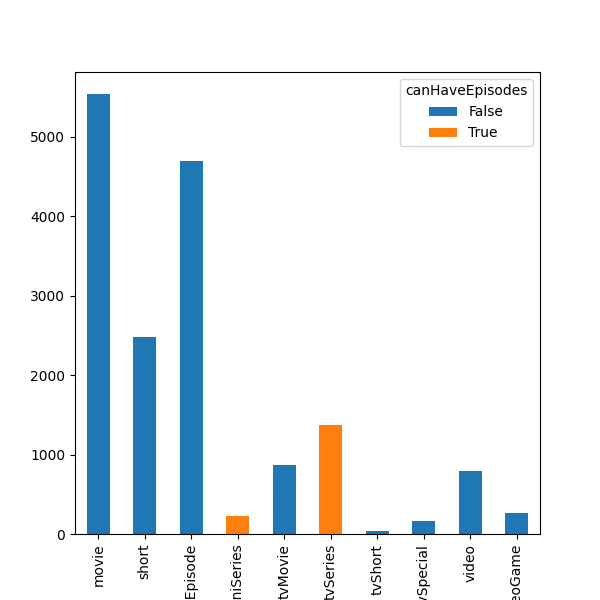
\includegraphics[width=\textwidth]{plots/fig1_a.png}
%         \caption{Counting of the title types frequencies combined with the canHaveEpisodes variable}
%         \label{fig:sub1}
%     \end{subfigure}
%     \subfigure[]{
%         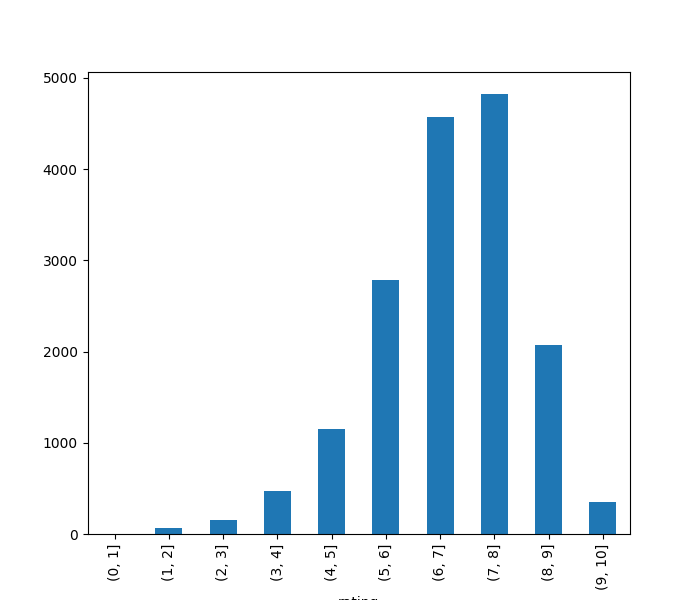
\includegraphics[width=0.48\textwidth]{plots/fig1_b.png}
%     }
%     \subfigure[]{
%         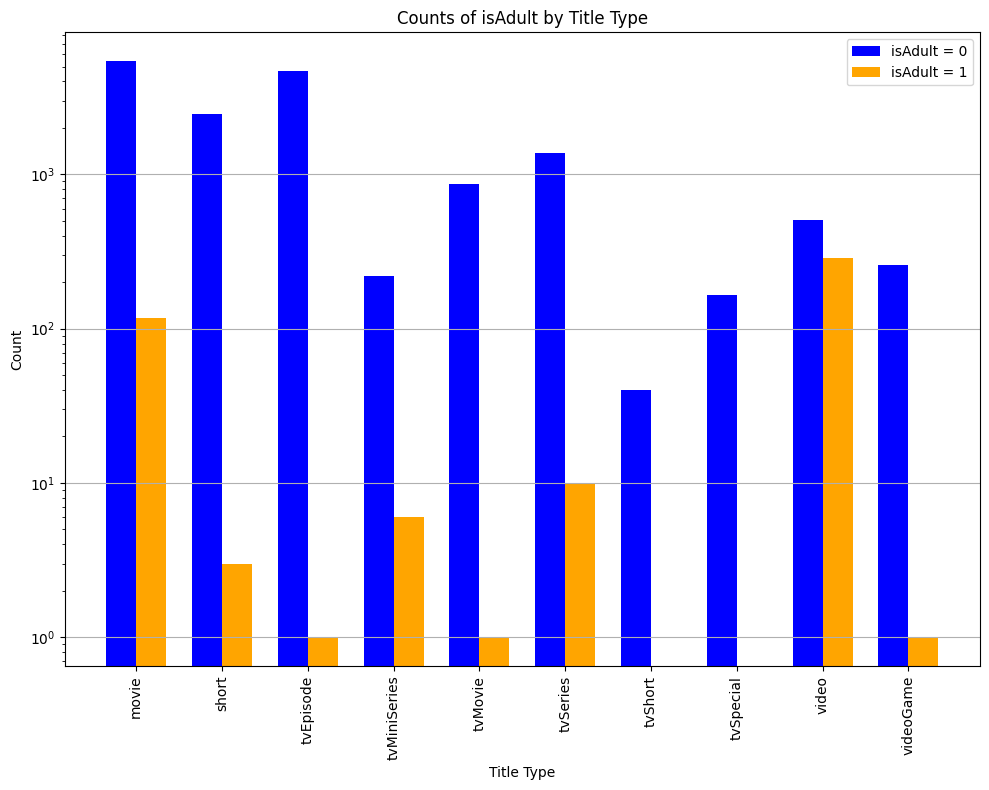
\includegraphics[width=0.48\textwidth]{plots/fig1_c.png}
%     }
%     \subfigure[]{
%         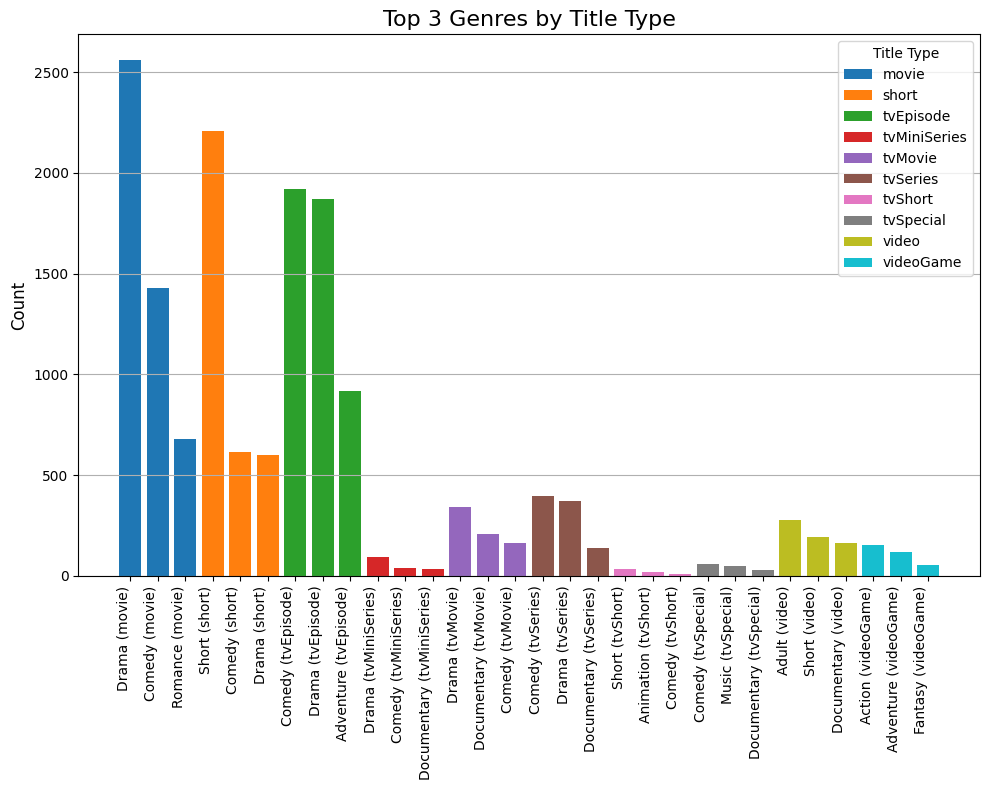
\includegraphics[width=0.48\textwidth]{plots/fig1_d.png} 
%     }
%     \caption{Bar chart of the discrete attributes
%     (b): counting of ratings frequencies;
%     (c): counting of the adult and non-adult frequencies combined with the
%     isRatable attribute;
%     (d) top 3 genres according to the titleType.}
%     \label{fig:bar-charts}
% \end{figure}


\begin{figure}[H]
    \centering
    % First subfigure
    \begin{subfigure}{0.48\textwidth}
        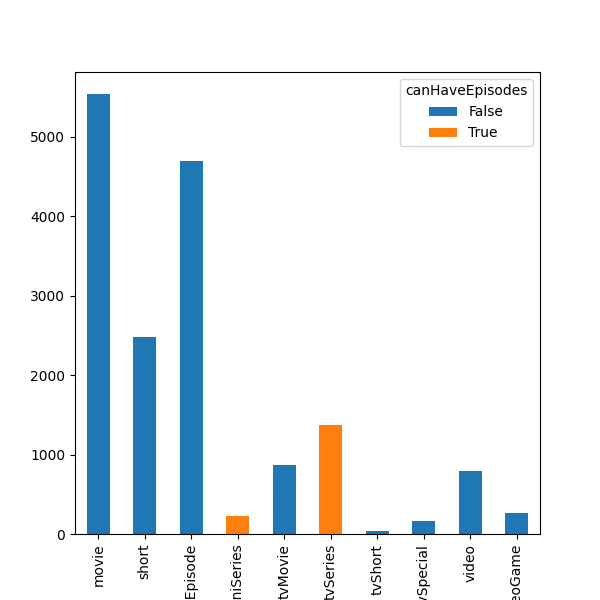
\includegraphics[width=\textwidth]{plots/fig1_a.png}
        \caption{Counting of the title types frequencies} %  combined with the canHaveEpisodes variable
        \label{fig:sub1}
    \end{subfigure}
    \hfill
    % Second subfigure
    \begin{subfigure}{0.48\textwidth}
        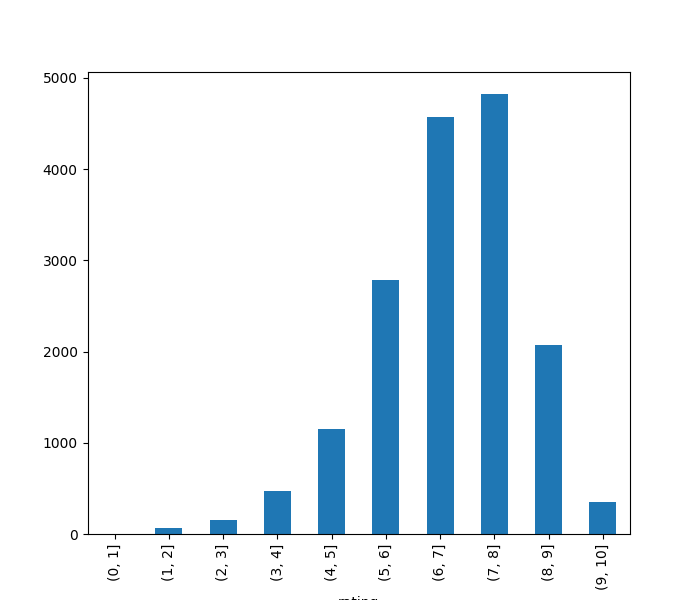
\includegraphics[width=\textwidth]{plots/fig1_b.png}
        \caption{Counting of ratings frequencies}
        \label{fig:sub2}
    \end{subfigure}
    
    % Third subfigure
    \begin{subfigure}{0.48\textwidth}
        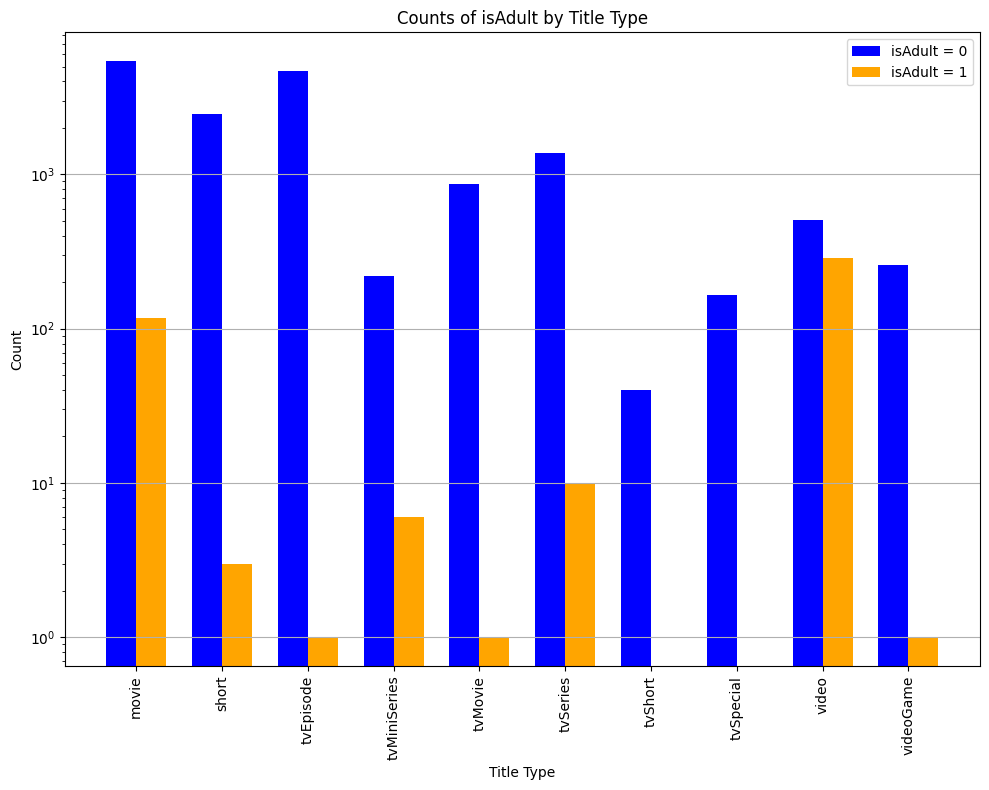
\includegraphics[width=\textwidth]{plots/fig1_c.png}
        \caption{Counting of the adult and non-adult per type}
        \label{fig:sub3}
    \end{subfigure}
    \hfill
    % Fourth subfigure
    \begin{subfigure}{0.48\textwidth}
        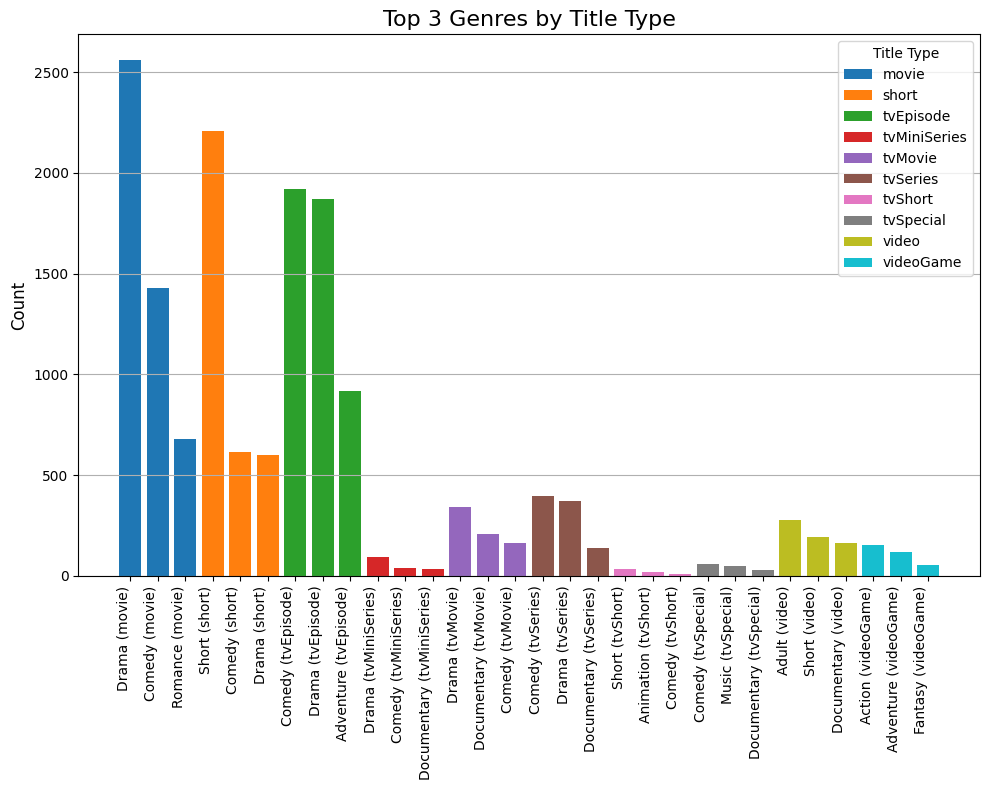
\includegraphics[width=\textwidth]{plots/fig1_d.png}
        \caption{types per genre}
        \label{fig:sub4}
    \end{subfigure}
    
    \caption{Bar chart of the discrete attributes.}
    \label{fig:bar-charts}
\end{figure}


\subsection{Variable elimination}\label{subsec:var_elim_discrete}
Because of redundancy and irrelevance, the following categorical variables were removed from the dataset:
\begin{itemize}
    \item \texttt{originalTitle} was removed because it is not relevant for the analysis;
    \item \texttt{isRatable} variable was removed because all the titles in the dataset are ratable;
\end{itemize}

Additionally, the \texttt{isAdult} feature is highly correlated with the presence or absence of
\textit{Adult} as a genre (16 records differ in the train set, 1 in the test set), so the two were merged
with a logical OR operation.


\subsection{Features transformations}
% \texttt{countryOfOrigin} and \texttt{genres} variables (datatypes: strings) were converted into 
% lists of strings to facilitate further analysis.
% This transformation was necessary because some records contain multiple genres or countries as values for
% these variables.
The attribute \texttt{rating} was converted into an ordinal variable by taking the upper bound of each rating
interval's string representation. This approach was chosen because the minimum rating is 1, meaning the
lowest interval corresponds only to ratings of 1. For consistency, the same transformation was applied
to all other intervals.\\

The attribute \texttt{genre} was represented through one-hot encoding. This generated 27 new attributes
(without counting the \textit{Adult} genre, mentioned in section~\ref{subsec:var_elim_discrete}).
Rows with no genres were assigned a vector of all zeros, indicating the absence of any genres.\\

% After that, multi-label one-hot encoding was applied to the
% \texttt{genres} column; each unique genre was represented as a binary feature, 
% allowing records that belong to multiple genres simultaneously to maintain this information.
The attribute \texttt{countryOfOrigin} was represented by grouping the countries by continent.
The following variables have been created: 
\begin{multicols}{2}
\begin{itemize}
    \item \texttt{countryOfOrigin\_AF} (Africa);
    \item \texttt{countryOfOrigin\_AS} (Asia);
    \item \texttt{countryOfOrigin\_EU} (Europe);
    \item \texttt{countryOfOrigin\_NA} (North America);
    \item \texttt{countryOfOrigin\_SA} (South America);
    \item \texttt{countryOfOrigin\_OC} (Oceania);
    \item \texttt{countryOfOrigin\_UNK} (Unknown country).
\end{itemize}
\end{multicols}

Each of the previous features provides the number of countries in the corresponding continent.
\texttt{countryOfOrigin\_UNK} is used to represent the strings that are not chategorized as being part of a
continent.\\

The feature \texttt{countryOfOrigin\_freq\_enc} is also created, providing the frequency encoding of the
original list as a whole. In summary, the original feature is represented by the listed 8 attributes.\\

This representation was chosen as it allows to keep a lot of the original information, while using
a small number of new features.\\




\section{Continuous attributes}
Table~\ref{tab:numerical_attributes} shows the continuous attributes of the dataset,
a brief description of each attribute and their type.
\begin{table}[h]
    \centering
    \begin{tabular}{|l|l|l|} % Using 'l' for left alignment of columns
        \hline
        \textbf{Attribute} & \textbf{Type} & \textbf{Description} \\ 
        \hline
        \texttt{worstRating} & Float & Worst title rating \\ 
        \hline
        \texttt{bestRating} & Float & Best title rating \\ 
        \hline
        \texttt{runtimeMinutes} & Integer & Runtime of the title expressed in minutes \\ 
        \hline
        \texttt{startYear} & Integer & Release/start year of a title \\ 
        \hline
        \texttt{endYear} & Integer & TV Series end year \\
        \hline
        \texttt{awardWins} & Integer & Number of awards the title won \\ 
        \hline
        \texttt{numVotes} & Integer & Number of votes the title has received \\ 
        \hline
        \texttt{totalImages} & Integer & Number of Images on the IMDb title page \\ 
        \hline
        \texttt{totalVideos} & Integer & Number of Videos on the IMDb title page \\ 
        \hline
        \texttt{totalCredits} & Integer & Number of Credits for the title \\ 
        \hline
        \texttt{criticReviewsTotal} & Integer & Total Number of Critic Reviews \\ 
        \hline
        \texttt{awardNominationsExcludeWins} & Integer & Number of award nominations excluding wins \\ 
        \hline
        \texttt{numRegions} & Integer & The regions number for this version of the title \\ 
        \hline
        \texttt{userReviewsTotal} & Integer & Number of User Reviews \\ 
        \hline
        \texttt{ratingCount} & Integer & The total number of user ratings for the title \\ 
        \hline
    \end{tabular}
    \caption{Description of continuous attributes}
    \label{tab:numerical_attributes}
\end{table}


\subsection{Variable elimination and creation}\label{sec:var_elim_creation}


% \begin{minipage}{0.48\textwidth}
% \centering
% 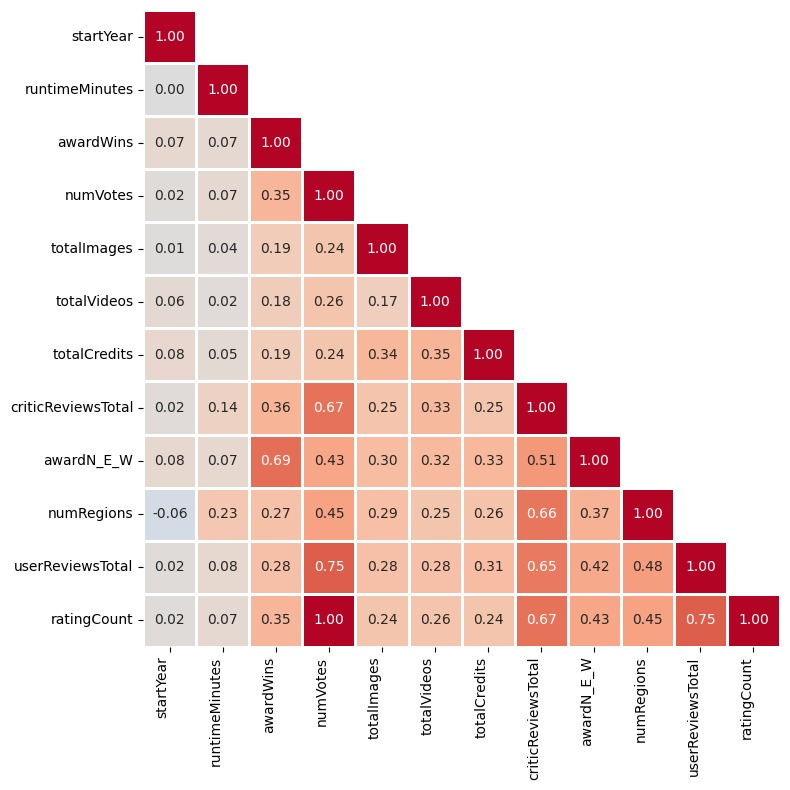
\includegraphics[width=0.6]{plots/correlation_matrix.png}
% \captionof{figure}{Correlation matrix}
% \label{fig:correlation_matrix} % Add a label for referencing
% \end{minipage}
\begin{figure}[H]
    \centering
    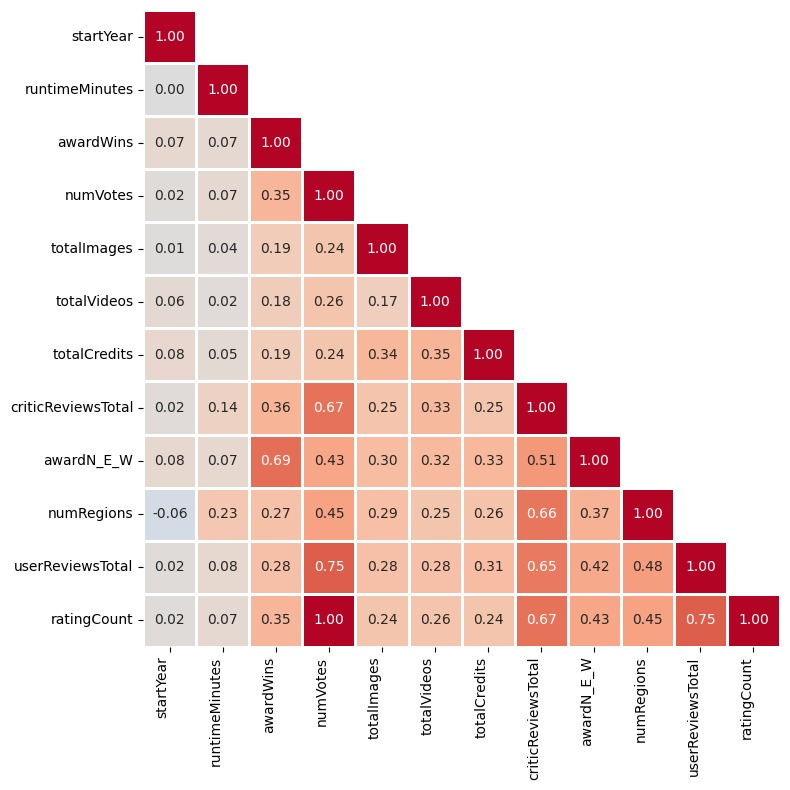
\includegraphics[width=0.6\textwidth]{plots/correlation_matrix.png}
    \caption{Correlation matrix of the numerical features}
    \label{fig:correlation_matrix}
\end{figure}

% \hfill
% \begin{minipage}{0.48\textwidth}
    The plot in figure~\ref{fig:correlation_matrix} is a Pearson's correlation matrix that takes into
    account the continuous variables of the dataset.
For what can be observed, \texttt{numVotes} and \texttt{ratingCount} have a perfect positive correlation, making it redundant to keep both of them.
For this reason it has been decided to drop \texttt{ratingCount}.
Another variable that was removed, but for different reasons, is \texttt{endYear}; as mentioned in the \textit{Missing Values} subsection, this variable was discarded due to the lack of reliable imputation methods for its numerous missing values.\\

On the other hand, regarding categorial attributes, after having analized all of them, \texttt{bestRating}, \texttt{worstRating}, and \texttt{isRatable} were discarded because 
they were found to have, as unique values, respectively 10, 1 and True, resulting in variables with a limited contribution based on their distributions.
% \end{minipage}
While examining the dataset, some variables were found to be redundant or irrelevant for the analysis.
Those variables were removed to simplify the dataset and improve the performance of the data mining
techniques.
The following variables were removed:

\begin{itemize}
    \item \texttt{isRatable}: this variable was removed because all the titles in the dataset are ratable;
    \item \texttt{ratingCount}: this variable was removed because it is perfectly correlated with the \texttt{numVotes} variable;
\end{itemize}


\section{Data Quality}\label{sec:data_quality}
In this phase, a proper evaluation of the observed data was conducted in preparation for the analysis.
Once having checked that there are no duplicates and no incomplete rows in the dataset, 
attention was given at identifying missing values and outliers within the columns.



\subsection{Syntactic Inconsistencies}
% In the exploration of the dataset it has been noticed that \texttt{awardWins} was the only feature having missing values marked with \texttt{NaN}.
% However, there were missing values also in other columns (\texttt{endYear}, \texttt{runtimeMinutes} and \texttt{genres}), 
% but they were indicated with the string "\textbackslash N".
% To avoid this inconsistency that might have caused problems during data preparation, these values have been replaced with \texttt{NaN}.
% By doing so, any cell in the \texttt{endYear}, \texttt{runtimeMinutes} and \texttt{genres} columns 
% that previously contained the string "\textbackslash N" is now considered a proper missing value, detectable and manageable using Pandas' functions.



\subsection{Missing Values}
Once having solved the above-mentioned inconsistency, the resulting total amount of the missing values are the following, 
also represented in percentages for a better understanding:
\begin{itemize}
    \item \texttt{endYear}: it is the feature with the highest number of NaN values (15617; about 95\%). For this reason and due to the lack of reliable imputation methods, the entire feature has been removed;
    
    \item \texttt{runtimeMinutes}: it has 4852 missing values (29.5\%) that have been handled in two
    different ways: Two imputation strategies were used: one leverages the titleType feature to guide
    the imputation,
    while the other imputes the missing values independently of any other features.
    Depending on the task at hand, one or the other was chosen;
    % by grouping the records by \texttt{titleType} and substituting the NaN value with the median of each group \textbf{ALTRIMENTI prendere valore random tra il 30\% - 70\% per titletype; anche se questo causa problemi nel momento in cui andiamo a classificare un nuovo record che non ha titletype};
    
    \item \texttt{awardWins}: this feature has 2618 NaN values (about 16\%). Since the mode associated with this variable is 0, it has been decided to substitute the missing values with 0;

    \item \texttt{genres}: it has 382 missing values (2.3\%). Having dealt this variable with a multi-label one-hot encoding process (as will be described in the \textit{Variable Transformation} section), a vector of all zeros is assigned to record with missing genres values.
\end{itemize}



\subsection{Outliers detection and variable Transformation}
% While examining the dataset, it became apparent that some attributes have outliers. 
% The important aspect to highlight is that since \texttt{awardWins}, \texttt{totalVideos} 
% and \texttt{awardNominationsExcludeWins} have many values as 0 (respectively 11971, 14821, 14427), 
% these might be considered variables with many outliers 
% (as seen in Figure \textbf{METTERE GRAFICO che rappresenti in qualche modo il result di DETECT\_OULIERS\_MULTI\_ATTRIBUTES in data\_quality noemi}) 
% but they actually have less outliers compared to the other variables.
For the other attributes \textbf{CONTINUARE......}
\textbf{VALORI OUTLIERS SU TRAIN IN \%: 86.7 , 90.2 , 87.8}
\textbf{VALORI OUTLIERS SU DF\_PP IN \%: 88.7 , 90.2 , 87.8}
Even though they are not proper outliers, the records that had "Videogame" as value of the attribute \texttt{titleType} were removed 
because of the fundamentally different titletype compared to the other title types of the dataset. In addition, their value of \texttt{runtimeMinutes}
seemed erroneous since they have an undefined or irrelevant runtime.


% \section{Variable Transformation}\label{sec:var_Transformation}
As a first step in the variable transformation process, the \texttt{countryOfOrigin} and \texttt{genres} variables (datatypes: strings) were converted into 
lists of strings to facilitate further analysis. This transformation was necessary because some records contain multiple genres or countries as values for these variables.
After that, multi-label one-hot encoding was applied to the \texttt{genres} column; each unique genre was represented as a binary feature, 
allowing records that belong to multiple genres simultaneously to maintain this information.
A similar approach was taken for the \texttt{countryOfOrigin} attribute; however, instead of creating a separate feature for each unique country 
(as there were many of them), countries were grouped by continent.
The following variables have been created: 
\begin{multicols}{2}
\begin{itemize}
    \item \texttt{countryOfOrigin\_NA} (North America);
    \item \texttt{countryOfOrigin\_SA} (South America);
    \item \texttt{countryOfOrigin\_AF} (Africa);
    \item \texttt{countryOfOrigin\_AS} (Asia);
    \item \texttt{countryOfOrigin\_EU} (Europe);
    \item \texttt{countryOfOrigin\_OC} (Oceania);
    \item \texttt{countryOfOrigin\_UNK} (Unknown continent).
\end{itemize}
\end{multicols}
% \begin{itemize}
%     \item \texttt{countryOfOrigin\_NA} (North America);
%     \item \texttt{countryOfOrigin\_SA} (South America);
%     \item \texttt{countryOfOrigin\_AF} (Africa);
%     \item \texttt{countryOfOrigin\_AS} (Asia);
%     \item \texttt{countryOfOrigin\_EU} (Europe);
%     \item \texttt{countryOfOrigin\_OC} (Oceania);
%     \item \texttt{countryOfOrigin\_UNK}.
% \end{itemize}
This transformation was implemented using \texttt{pycountry\_convert}, a Python library that converts between different country and continent codes and names. 
Its function \texttt{country\_alpha2\_to\_continent\_code()} was used to process the lists of strings of the \texttt{countryOfOrigin} variable;
the function takes a country code in the ISO 3166-1 alpha-2 format (e.g., "US", "FR", "IN") and returns the corresponding continent code. 
If the country code is invalid or there are obsolete country names, the \texttt{countryOfOrigin\_UNK} variable gets a value according to the number of unknown countries for that record. 
For each record, these new variables contain counts representing the number of countries from each continent.
In addition, \texttt{countryOfOrigin\_freq\_enc} was created to capture frequency-based information. 
Unlike the continent-based variables that count individual countries, this variable represents how frequently a specific combination of countries appears across the entire dataset.\\
% Six binary attributes were created: \texttt{is\_from\_Africa}, \texttt{is\_from\_Asia}, \texttt{is\_from\_Europe}, \texttt{is\_from\_North America}, \texttt{is\_from\_Oceania}, and \texttt{is\_from\_South America}.
% This transformation preserves information about titles produced in more than one continent, as they will have a value of 1 for each corresponding attribute.
Furthermore, it has been decided to extract the ceiling value for each entry in the \texttt{rating} column, in order to use it as an integer for further analysis.\\
Looking at the already existing features it has also been decided to aggregate some of them in order to create more stable and meaningful data. 
In particular, \texttt{awardWins} and \texttt{awardNominationsExcludeWins} were combined into a new variable called \texttt{totalNominations} to take into account
which records have received a nominations, independently from the fact that they then won or not.
Two other variables, i.e. \texttt{totalImages} and \texttt{totalVideos} were aggregated into \texttt{totalMedia} to sum the number of multimedia elements
of each record.\\

As for the continuous attributes, it was observed that they required a stronger transformation due to their highly positively skewed distributions. 
Specifically, when required by the data mining method, a log-transformation was applied to all the numeric attributes, since their skewness was highly greater than 1. 
Following the log-transformation, standard normalization techniques - \texttt{MinMaxScaler} and \texttt{StandardScaler} - have then been applied (when scaling was necessary); 
respectively to scale each feature to a given range and to standardize features by removing the mean and scaling to unit variance.
The decision to apply one or the other was again made based on the specific requirements of each data mining technique, and so will be specified accordingly in each section.
\textbf{CONTROLLARE SE IN OGNI SEZIONE C'E' SPECIFICA SULLE DUE NORMALIZZAZIONI USATE!!!}.


% \section{Pairwise correlations and elimination of variables}\label{sec:correlation}
% %The plot in figure~\ref{fig:correlation_matrix} is a Pearson's correlation matrix that takes into account the continuous variables of the dataset.
% % For what can be observed, \texttt{numVotes} and \texttt{ratingCount} have a perfect positive correlation, making it redundant to keep both of them.
% % For this reason it has been decided to drop \texttt{ratingCount}.
% % Another variable that was removed, but for different reasons, is \texttt{endYear}; as mentioned in the \textit{Missing Values} subsection, this variable was discarded due to the lack of reliable imputation methods for its numerous missing values.\\

% % On the other hand, regarding categorial attributes, after having analized all of them, \texttt{bestRating}, \texttt{worstRating}, and \texttt{isRatable} were discarded because 
% % they were found to have, as unique values, respectively 10, 1 and True, resulting in variables with a limited contribution based on their distributions.

% % \begin{figure}[h!] % Positioning options: h (here), t (top), b (bottom), p (page)
% %     \centering % Centers the figure
% %     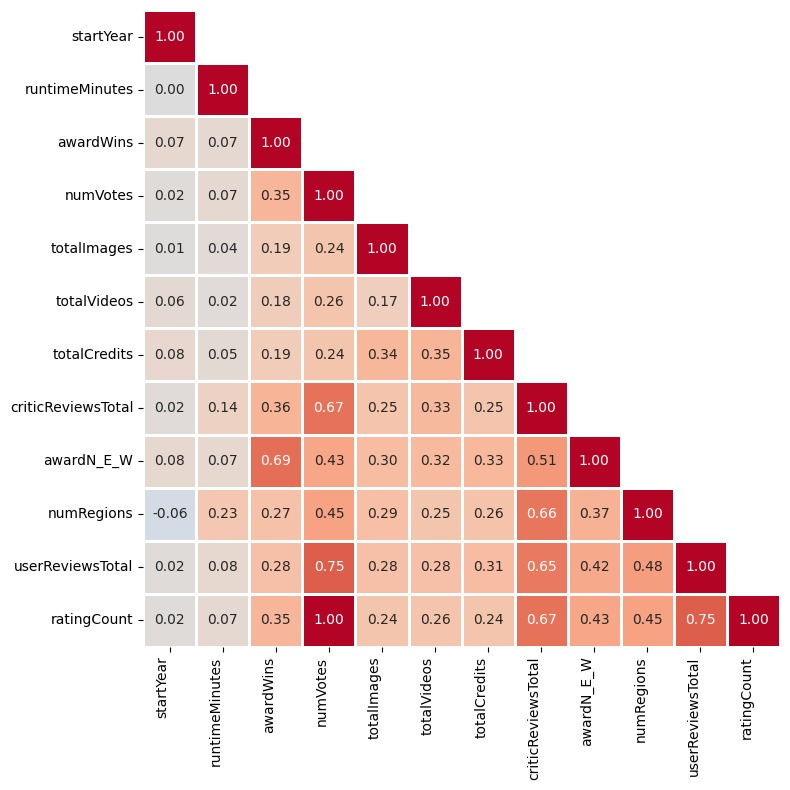
\includegraphics[width=0.7\textwidth]{plots/correlation_matrix.png} % Specify the file name and scaling options
% %     \caption{Correlation matrix} % Add a caption
% %     \label{fig:correlation_matrix} % Add a label for referencing
% % \end{figure}

% \noindent
% \begin{minipage}{0.48\textwidth}
%     \centering
%     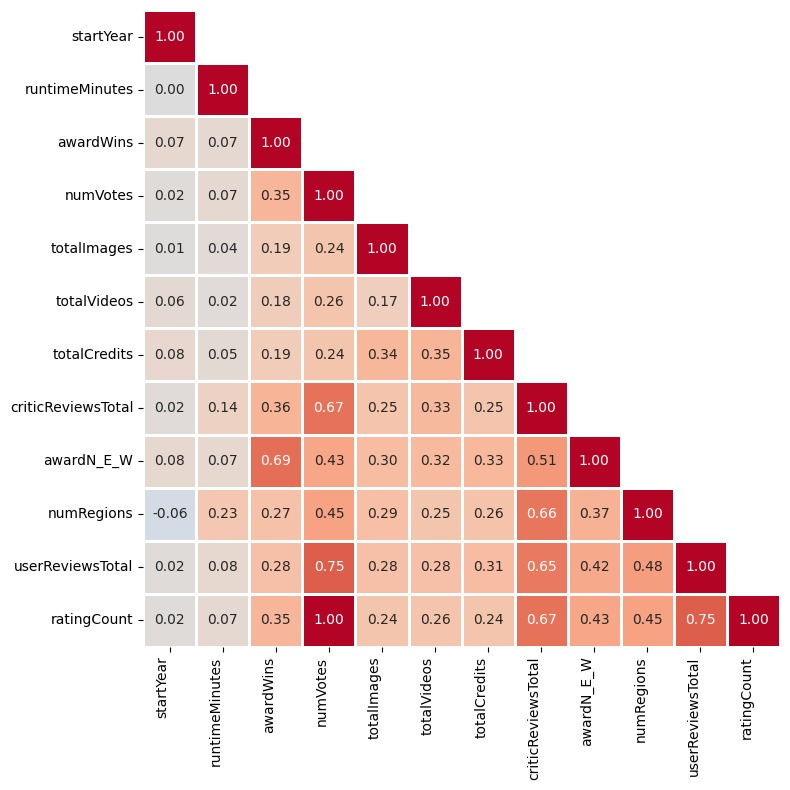
\includegraphics[width=\linewidth]{plots/correlation_matrix.png}
%     \captionof{figure}{Correlation matrix}
%     \label{fig:correlation_matrix} % Add a label for referencing
% \end{minipage}
% \hfill
% \begin{minipage}{0.48\textwidth}
%     The plot in figure~\ref{fig:correlation_matrix} is a Pearson's correlation matrix that takes into account the continuous variables of the dataset.
% For what can be observed, \texttt{numVotes} and \texttt{ratingCount} have a perfect positive correlation, making it redundant to keep both of them.
% For this reason it has been decided to drop \texttt{ratingCount}.
% Another variable that was removed, but for different reasons, is \texttt{endYear}; as mentioned in the \textit{Missing Values} subsection, this variable was discarded due to the lack of reliable imputation methods for its numerous missing values.\\

% On the other hand, regarding categorial attributes, after having analized all of them, \texttt{bestRating}, \texttt{worstRating}, and \texttt{isRatable} were discarded because 
% they were found to have, as unique values, respectively 10, 1 and True, resulting in variables with a limited contribution based on their distributions.
% \end{minipage}